\documentclass[
  parskip=half,
  bibliography=totoc,     % Literatur im Inhaltsverzeichnis
  captions=tableheading,  % Tabellenüberschriften
  titlepage=firstiscover, % Titelseite ist Deckblatt
]{scrartcl}
%
% LaTeX2e korrigieren.
\usepackage{fixltx2e}
% Warnung, falls nochmal kompiliert werden muss
\usepackage[aux]{rerunfilecheck}
%
\usepackage{blindtext}
% deutsche Spracheinstellungen
\usepackage{polyglossia}
\setmainlanguage{german}
%
% unverzichtbare Mathe-Befehle
\usepackage{amsmath}
% viele Mathe-Symbole
\usepackage{amssymb}
% Erweiterungen für amsmath
\usepackage{mathtools}
%
% Fonteinstellungen
\usepackage{fontspec}
\defaultfontfeatures{Ligatures=TeX}
%
\usepackage[
  math-style=ISO,    % \
  bold-style=ISO,    % |
  sans-style=italic, % | ISO-Standard folgen
  nabla=upright,     % |
  partial=upright,   % /
]{unicode-math}
%
% Warnung! Bei Aktivierung der alternativen mathfonts (nächsten drei Befehle) 
% könnte die math-Umgebung nicht mehr funktionieren. -Arne
\setmathfont{Latin Modern Math}
\setmathfont[range={\mathscr, \mathbfscr}]{XITS Math}
\setmathfont[range=\coloneq]{XITS Math}
\setmathfont[range=\propto]{XITS Math}
% make bar horizontal, use \hslash for slashed h
\let\hbar\relax
\DeclareMathSymbol{\hbar}{\mathord}{AMSb}{"7E}
\DeclareMathSymbol{ℏ}{\mathord}{AMSb}{"7E}
%
% richtige Anführungszeichen
\usepackage[autostyle]{csquotes}
%
% Zahlen und Einheiten
\usepackage[
  locale=DE,                   % deutsche Einstellungen
  separate-uncertainty=true,   % Immer Fehler mit \pm
  per-mode=symbol-or-fraction, % m/s im Text, sonst Brüche
]{siunitx}
%für schöne Mengenangaben
\usepackage{dsfont}
% chemische Formeln
\usepackage[version=3]{mhchem}
%
% schöne Brüche im Text
\usepackage{xfrac}
%
% Floats innerhalb einer Section halten
\usepackage[section, below]{placeins}
% Captions schöner machen.
\usepackage[
  labelfont=bf,        % Tabelle x: Abbildung y: ist jetzt fett
  font=small,          % Schrift etwas kleiner als Dokument
  width=0.9\textwidth, % maximale Breite einer Caption schmaler
]{caption}
% subfigure, subtable, subref
\usepackage{subcaption}
%
% Grafiken können eingebunden werden
\usepackage{graphicx}
% größere Variation von Dateinamen möglich
\usepackage{grffile}
%
% Standardplatzierung für Floats einstellen
\usepackage{float}
\floatplacement{figure}{h}
\floatplacement{table}{h}
%
% schöne Tabellen
\usepackage{booktabs}
%
% Seite drehen für breite Tabellen
\usepackage{pdflscape}
%
% Literaturverzeichnis
\usepackage[style=numeric,backend=biber]{biblatex}
% Quellendatenbank
\addbibresource{lit.bib}
\addbibresource{programme.bib}
%
% Hyperlinks im Dokument
\usepackage[
  unicode,
  pdfusetitle,    % Titel, Autoren und Datum als PDF-Attribute
  pdfcreator={},  % PDF-Attribute säubern
  pdfproducer={}, % "
]{hyperref}
% erweiterte Bookmarks im PDF
\usepackage{bookmark}
%
% Trennung von Wörtern mit Strichen
\usepackage[shortcuts]{extdash}
%
\author{
  Helena Nawrath
  \texorpdfstring{
    \\
    \href{mailto:helena.nawrath@tu-dortmund.de}{helena.nawrath@tu-dortmund.de}
  }{}%
  \texorpdfstring{\and}{, }
  Carl Arne Thomann
  \texorpdfstring{
    \\
    \href{mailto:arnethomann@me.com}{arnethomann@me.com}
  }{}
}
\publishers{TU Dortmund – Fakultät Physik}

%%% Hier definiert man Titel, Autor und Datum %%%%%%%%%%%%%%%%%%%%%%%%%%%%%%%%%

\subject{Versuch 204}
\title{Wärmeleitfähigkeit von Metallen}
\date{
  Durchführung: 04.11.2014
  \hspace{3em}
  Abgabe: 11.11.2014
}

%%%%%%%%%%%%%%%%%%%%%%%%%%%%%%%%%%%%%%%%%%%%%%%%%%%%%%%%%%%%%%%%%%%%%%%%%%%%%%%

\begin{document}

\maketitle
\thispagestyle{empty}
\newpage

\section{Zielsetzung}

Versuchsziel ist es, sich mit der Funktionsweise des Lock-In-Verstärkers vertraut zu machen. 
Außerdem soll für 10 verschiedene Phasen mit und ohne verrauschtes Signal die Funktionsweise verifiziert werden. 
Zuletzt soll die Rauschunterdrückung mit einer Photodetektorschaltung überprüft werden.

\section{Theorie}
\label{sec:Theorie}
Lock-In-Verstärker werden eingesetzt, um Signale mit hohem Rauschen zu messen. 
%Im Gegensatz zum Bandpass kann hier auch Rauschen herausgefiltert werden, welches auf der selben Frequenz wie das Messsignal liegt.
%
Das zu messende Eingangssignal $U_\mathup{sig}$ durchläuft im Gerät verschiedene Bauelemente, die in Abbildung \ref{fig:lockin} dargestellt sind.
\begin{figure}
	\centering
		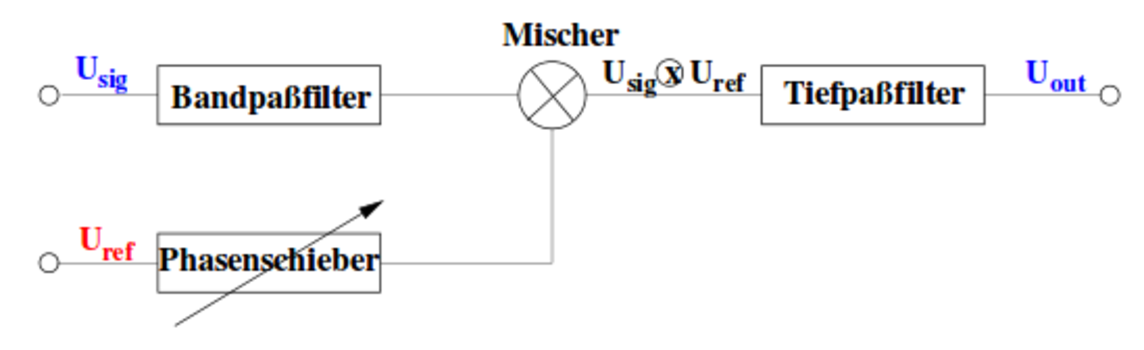
\includegraphics[width=0.7\textwidth]{Bilder/LOCK_IN.pdf}
		\caption{Schematischer Aufbau des Lock-In-Verstärkers. \cite{V303}}
		\label{fig:lockin}
	\end{figure}

Nach der Verstärkung durch den \enquote{Pre-Amplifier} durchläuft das Signal zunächst einen \enquote{Bandpassfilter}, der das Rauschen minimiert. 
Alle Frequenzen $\omega<<\omega_0$ und $\omega>>\omega_0$ werden grob herausgefiltert.
Ein \enquote{Funktionsgenerator} erzeugt die Referenzspannung $U_\mathup{ref}$ -- eine Sinus- oder Rechteckspannung der Frequenz $\omega_0$ -- , welche über den \enquote{Phasenschieber} an die Phase des Eingangssignals angepasst werden kann. 
Dieser Vorgang nennt sich Synchronisation.
Im \enquote{Mischer} treffen beide Signale aufeinander und werden multipliziert. 
Anschließend wird das Mischsignal $U_\mathup{sig}\times U_\mathup{ref}$ an den \enquote{Tiefpass} weitergeleitet, der die Modulationsfrequenz $\omega_0$ über mehrere Perioden integriert, um restliche Rauschanteile $\omega\neq\omega_0$ auszuschließen. 
Zurück bleiben nur die Anteile der Signalsspannung $U_\mathup{sig}$, die mit der Referenzspannung synchronisiert werden konnten.
Um eine möglichst geringe Bandbreite $\Delta{\nu}=\frac{1}{\pi RC}$ zu erhalten, sollte die Zeitkonstante $\uptau=RC$ des \enquote{Tiefpasses} ausreichend groß gewählt werden. 
Damit wird eine hohe Güteziffer im Bezug auf Störungsfilterung erzielt.

Die Ausgangsspannung $U_\mathup{out}$ ist eine Gleichspannung, welche proportional zur Eingangsspannung $U_\mathup{sig}$ und zum Cosinus der Phasendifferenz $\Delta\Phi$ ist:
\begin{equation}
 	U_\mathup{out}\propto{U_\text{sig}}\text{cos}(\Delta\Phi). 
 	\label{cosinus_ausgangsspannung}
 \end{equation} 
$U_\mathup{out}$ wird also maximal, wenn die Phasendifferenz $\Delta\Phi=0$ (wahlweise Vielfache von 180°) beträgt. \cite{regensburg}
%Quellenangabe http://www.physik.uni-regensburg.de/studium/praktika/a2/download/versuch5a.pdf

\begin{figure}
	\centering
		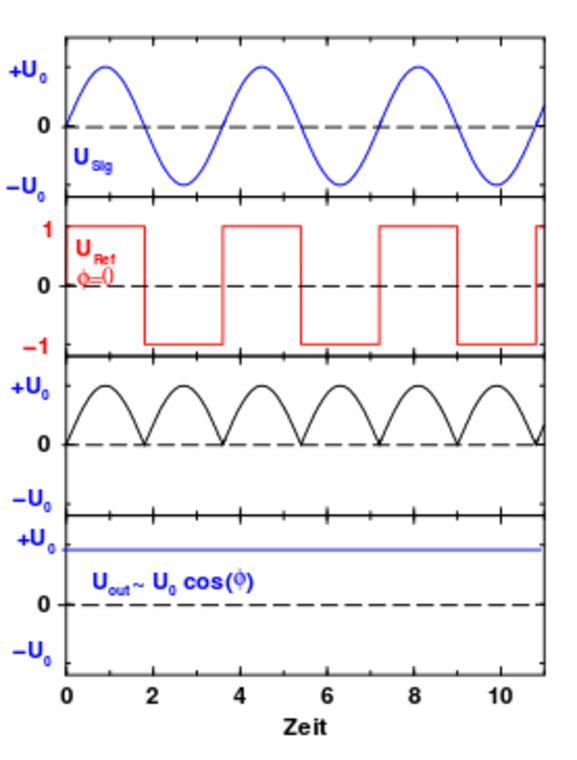
\includegraphics[width=0.4\textwidth]{Bilder/Beispiel.pdf}
		\caption{Überlagerung eines sinusförmigen Eingangssignals mit rechteckiger Referenzsspannung. \cite{V303}}
		\label{fig:bsp}
	\end{figure}
Wird beispielsweise ein sinusförmiges Eingangssignal $U_\mathup{sig}=U_0sin(\omega t)$ wie in Abbildug \ref{fig:bsp} mit einem rechteckigen Referenzsignal $U_\mathup{ref}$ gleicher Frequenz überlagert, wird diese zunächst durch eine Fourierreihe angenähert, welche aus den ungeraden Harmonischen der Grundfrequenz besteht. 
Wird das multiplizierte Signal,  bestehend aus geraden Oberwellen der Frequenz $\omega$ durch den als Gleichrichter funktionierenden Tiefpass geleitet ergibt sich die Gleichspannung
\begin{equation}
	U_\mathup{out}=\frac{2}{\pi}U_0\text{cos}(\Phi).
\end{equation}
Besteht kein Phasenunterschied zwischen Eingangs- und Referenzsignal nimmt die Ausgangsspannung ihren Maximalwert 
\begin{equation}
	U_\mathup{out}=\frac{2}{\pi}U_0
\end{equation}
an.
Die Rechteckspannung mit auf 1 genormter Amplitude realisiert einen Schalter (\enquote{Chopper}). 
Indem die Werte 1 und -1 durch positive und negative Halbwellen angenommen werden, steht der Schalter auf \enquote{Ein} bzw. \enquote{Aus}.




\section{Durchführung}
\label{sec:Durchfuehrung}
\subsection{Freie Schwingung mit Dämpfung}
Im ersten Teil wird die freie, gedämpfte Schwingung mit einem Serienschwingkreis untersucht.
Es wird die Zeitabhängigkeit der Kondensatorspannung $U_\mathup{C}(\omega, t)$ betrachtet und ihr Verlauf diskutiert.
Hierzu wird eine Schaltung wie in Abbildung \ref{fig:schaltkreis_erzwungen} angesetzt.
Der Generator wird auf Rechteckspannung mit einer solch geringen Frequenz $f$ eingestellt, dass innerhalb einer Periode des Generator das System frei oszillieren und abklingen kann, ehe es nach der Periodendauer $\frac{1}{f}$ erneut angeregt wird.
Die weiteren Systemparameter, etwa die Komponenten des Schwingkreises, werden so gewählt, dass die charakteristischen Verläufe sichtbar werden. 
Die Verläufe der Kondensatorspannung $U_\mathup{C}(\omega, t)$ werden dargestellt und gespeichert.

Die systembeschreibende Abklingzeit $T_\text{ex}$ wird an diesen Verläufen bestimmt und mit dem vorhergesagten Wert nach der Gleichung \eqref{eq:abkling} verglichen.\\
Der aperiodische Grenzfall wird als Grenze zwischen Kriechfall und Schwingfall mittels Bisektion des Dämpfungswiderstandes $R$ angenähert, wozu der Schwingkreis mit einem variablen Widerstand ausgestattet wird.
Der auf diese Weise ermittelte Dämpfungswiderstand $R_\text{ap}$ wird mit dem theoretischen Wert $R_\text{ap,t}$ aus \ref{sec:theorie1} verglichen.

\subsection{Erzwungene Schwingung mit Dämpfung}
Im zweiten Teil wird die erzwungene, gedämpfte Schwingung untersucht.
Gemessen wird die Frequenzabhängigkeit der Kondensatorspannung $U_\mathup{C}(\omega, t)$ eines Serienschwingkreises sowie der Phasenwinkel $\phi$ zwischen der Erregerspannung $U(t)$ und der Kondensatorspannung $U_\mathup{C}(\omega, t)$.\\
Hierzu wird einerseits bei verschiedenen Erregerfrequenzen $U(t)$  der Betrag der Kondensatorspannung $U_\mathup{C}(\omega, t)$ und die Zeitdifferenz der Nulldurchgänge von Erregerspannung $U(t)$ und von der Kondensatorspannung $U_\mathup{C}(\omega, t)$ betrachtet.
Weiter wird zur Charakterisierung des Resonanzverhaltens die Güte $q$ und die Resonanzbreite $\mathup{\Delta}\, f$ bestimmt.

% Ein Wanderurlaub im ehemaligen Jugoslawien. Klingt zunächst einmal furchtbar spannend, ist aber eigentlich der Gähner (=Langeweiler, langweilige Sache) überhaupt.

% Jeder denkt: Alte Militärbaracken, Herrenausstatter wohin man schaut, vielleicht ein Museum für altertümliche Fahrstuhltechnik, klingt doch toll! Doch hält diese vorgefasste Meinung einer genaueren Betrachtung nicht stand. Schon morgens im Hotel wird die Kehrseite der Medaille deutlich:

% Aufzug defekt. Buffet unvollständig. Chinesische Loungemusik. Despotisches Hotelpersonal. Eierlikör ausverkauft. Französischer Kofferträger. Gewaltsamer Raubüberfall. Hasenzähnige Empfangsdame. Interplanetarer Schmugglerstützpunkt. Jodelmusikkorps nebenan. Kreditkarte gesperrt. Lilafarbener Teppichläufer. Monochromatisches Licht. Nucleophile Substitution. Ortsunkundige Japaner. Präsidentenleiche unübersehbar. Qualmender Ethanolofen. Resistiver Touchscreen. Systematische Tötungen. Trauriger Clown. Unerfreuliche Massenbegräbnisse. Verwanzte Matratzen. Wadenkrampffördernde Beleuchtung. X-Beinige Pianodame. Yorkshireterrier bellt. Bezahlung nur bar möglich (und nicht per EC-Karte, wie ich es sonst immer mache).

% Also merke: Der Spruch „Im Norden geht die Sonne auf, im Süden nimmt sie Ihren Lauf, […] Westen wird sie untergehen, usw.“, gilt nicht wenn man auf dem Mond (oder einem anderen Erdtrabanten) steht (oder sitzt, außer man liegt).

\section{Auswertung}
\label{sec:Auswertung}
\begin{table}
	\centering
	\begin{tabular}{S[table-format=2.0] S[table-format=3.0] S[table-format=3.0] S[table-format=2.2]}
	\toprule
{$n$} & {$U_n/\:\si{\milli{\volt}}$} & {$\frac{U_1}{n}/\:\si{\milli{\volt}}$} & {Abweichung in $\%$}\\
	\midrule
 1 & 920 & 912 &  1\\
 3 & 300 & 288 &  4\\
 5 & 170 & 168 &  1\\
 7 & 116 & 112 &  4\\
 9 &  86 &  80 &  8\\
11 &  64 &  56 & 14\\
	\bottomrule
	\end{tabular}
	\caption{Fourieranalyse der Rechteckspannung.}
	\label{tab:FA_RE}
\end{table}
 
\begin{table}
	\centering
	\sisetup{table-format=2.3}
	\begin{tabular}{S[table-format=2.0] S[table-format=3.0] S[table-format=3.1] S[table-format=1.2] }
	\toprule
	{$n$} & {$U_n/\:\si{\milli\volt}$} & {$\frac{U_1}{n}/\:\si{\milli\volt}$} & {Abweichung in $\%$}\\
	\midrule
 1 & 580 & 576.0 & 0.7\\
 3 &  63 &  61.6 & 2.3\\
 5 &  21 &  20.8 & 1.0\\
 7 &  10 &  10.4 & 3.9\\
 9 &   6 &   5.6 & 7.1\\
11 &   4 &   4.0 & 0.0\\
	\bottomrule
	\end{tabular}
	\caption{Fourieranalyse der Dreiecksspannung.}
	\label{tab:FA_RE}
\end{table}



\begin{table}
	\centering
	\sisetup{table-format=2.3}
	\begin{tabular}{S[table-format=2.0] S[table-format=3.0] S[table-format=3.1] S[table-format=1.0] }
	\toprule
	{$n$} & {$U_n/\:\si{\milli\volt}$} & {$\frac{U_1}{n}/\:\si{\milli\volt}$} & {Abweichung in $\%$}\\
	\midrule
 1 & 460 & 456 & 1\\
 2 & 230 & 224 & 3\\
 3 & 152 & 144 & 6\\
 4 & 112 & 112 & 0\\
 5 &  88 &  88 & 0\\
 6 &  74 &  74 & 0\\
 7 &  64 &  64 & 0\\
 8 &  56 &  56 & 0\\
 9 &  50 &  48 & 4\\
10 &  44 &  46 & 5\\
11 &  40 &  40 & 0\\
	\bottomrule
	\end{tabular}
	\caption{Fourieranalyse der Sägezahnspannung.}
	\label{tab:FA_RE}
\end{table}



\section{Diskussion}
\label{sec:Diskussion}

\subsection{Fehlerdiskussion}
Für die Fehlerdiskussion verwertbare Messwerte wurden in Abschnitt \ref{sec:Auswertung2}, Tabelle \ref{tab:block_messung} sowie in Abschnitt \ref{sec:Auswertung3}, Tabelle \ref{tab:auge} beschrieben.
Für die Bestimmung dieser Messwerte wurde der Betrag der Schallgeschwindigkeit in Abschnitt \ref{sec:Auswertung1}, Gleichung \eqref{qu:geschwindigkeit} gefunden.
Die geringe Abweichung von dem Literaturwert bezeugt, dass es nicht zu systematischen Fehlern kam und das Grundprinzip der Messung ein zuverlässiges Ergebnis liefert.

Die starken Abweichungen bei der Bestimmung der Materialfehler $a$ im Block von bis zu $27\%$ und 
bei der Bestimmung des Lochdurchmessers $d$ von bis zu $233\%$.
Die starke Abweichung in der Unsicherheit im Laufe der Messung weist auf starke statistische Fehler und eine ungeeignete Wahl der Schallfrequenz hin. 
Die Maßstäbe des Augenmodells, das als brauchbares $1$:$3$-Modell angenommen wird, wurden mit starker Abweichung von der Literaturangabe bestimmt.
Dies weist ähnlich zum vorangegangen Fall auf ungeeignete Wahl der Frequenz hin.

\subsection{Verwendung des Ultraschall-Verfahrens}
Es konnte im Experiment die Anwendbarkeit des Ultraschall-Verfahrens zur Feststellung von Materialfehlern und, bei geeignetem Aufbau sowie geeigneter Wahl der Einstellungen, die Tiefenauflösung nachgewiesen werden.
Das Prinzip ist somit in Industrie zur zerstörungsfreien Fehlerprüfung und in der Medizin zur nicht-invasiven Maßnahme als bildgebendes Verfahren verwendbar.
%\nocite{Versuchsnummer}
\printbibliography
\noindent Die verwendeten Plots wurden mit \textit{matplotlib}\cite{matplotlib} und die Grafiken mit \textit{GIMP}\cite{gimp} erstellt sowie die Berechnungen mit Python-\textit{Python-Numpy}, \cite{numpy}, \textit{Python-Scipy}\cite{scipy} und \textit{Python-uncertainties}\cite{uncertainties} durchgeführt.
\end{document}
